\documentclass[11pt,onecolumn,oneside]{article}

\usepackage{amsmath, amssymb, amsfonts, bm}
\usepackage{newapa}
\usepackage{natbib}
\usepackage[dvips]{graphicx}

\newcommand{\pdiff}[2]{\frac{\partial #1}{\partial #2}}

\title{Curvature effects on the Sawyer-Eliassen Equation}
\author{Marshall Ward}

\begin{document}

\maketitle

\begin{center}{\large \bf Abstract}\end{center}

{\small We consider the effects of a tropopause that varies from a horizontal state. We still focus on a rigid, impermeable tropopause in steady-state flow, but wedetermine analytic solutions of the flow for the cases where it slopes or has constant curvature. While we do not the address the physical possibility of such a state, we demonstrate that these scenarios can be treated analytically, which may aid in numerical accuracy for more realistic treatments.}

\section{Introduction}

While most theoretical problems involving the tropopause approximate it as a rigid horizontal upper boundary, the true tropopause is not bound by such a restriction. It typically exhibits a nonuniform structure and can even reach the surface in extreme situations.

Such a variable boundary would be difficult to incorporate into most analytical problems. In the calculation of frontal flows however, the problem is essentially reduced to solving Poisson's equation. Countless methods have been developed over the years to solve this equation for nonuniform boundaries. We shall exploit a number of these methods in order to develop solutions for horizontal variation. Specifically, we consider the effects due to constant slope and constant curvature.

We first present a derivation of the Sawyer-Eliassen equations based on that of \citet{Hoskins:1982}, followed by a derivation of the solution for a sloping boundary for cases where the method of images is applicable. We then show how conformal mapping may be used to determine an analytic solution for a boundary of constant curvature. Finally, possible applications and future work are discussed. Much of the work here was inspired by and closely follows the work of \citet{Hakim+:2001}.

%%%%%%%%%%%%%%%%%%%%%%%%%%%%%%%%%%%%%%%%%%%%%%%%%%%%%%%%%%%%%%%%%%%%%%%%%%%%%%%%
%%%%%%%%%%%%%%%%%%%%%%%%%%%%%%%%%%%%%%%%%%%%%%%%%%%%%%%%%%%%%%%%%%%%%%%%%%%%%%%%

\section{Frontogenesis and the Sawyer-Eliassen Equation}

Fundamentally, frontogenesis refers to the localized buildup of sharp gradients in the atmosphere, typically for quantities such as buoyancy or potential temperature. In this section, we first consider the kinematics of frontogenesis, and then proceed to examine the dynamics in both the quasigeostrophic and the semigeostrophic approximations. Both cases will yield an equation for the vertical circulation, known as the Sawyer-Eliassen equation, which is equivalent to Poisson's equation under a coordinate transformation. Our study will then focus on solutions to this equation.

%%%%%%%%%%%%%%%%%%%%%%%%%%%%%%%%%%%%%%%%%%%%%%%%%%%%%%%%%%%%%%%%%%%%%%%%%%%%%%%%

\subsection{Kinematics of Frontogenesis}

We first consider the kinematics of some conserved quantity $b$, which will eventually be treated as the buoyancy, in an incompressible 2D flow. Then $b$ satisfies the equation
\begin{equation}\label{ConservedParcel}
\frac{Db}{Dt} = \pdiff{b}{t} + u \pdiff{b}{x} + v \pdiff{b}{y} = 0.
\end{equation}

We are essentially interested in the quantity $|\nabla b|$, which can be shown to satisfy the relation
\[
\frac{D}{Dt} |\nabla b|^2 = D |\nabla b|^2 \cos 2\phi,
\]
where $D$ is the so-called ``deformation'' along the dilatation axis and $\phi$ is the angle between the dilatation axis and the contours of $b$. Frontogenesis is typically associated with an increase of $|\nabla b|$, while frontolysis is associated with its decrease.

However, more information can be obtained by taking an alternative approach. Instead of focusing on the magnitude of the gradient of $b$, consider the evolution of the true gradient in the $x$-direction, $\frac{D}{Dt} \left( \pdiff{b}{x} \right)$, which can be written as
\[ \begin{split}
\frac{D}{Dt}\left(\pdiff{b}{x}\right) &= \pdiff{}{t} \pdiff{b}{x} + u \pdiff{}{x} \pdiff{b}{x} + v \pdiff{}{y} \pdiff{b}{x} \\
 &= \pdiff{}{x} \left(\pdiff{b}{t} + u \pdiff{b}{x} + v \pdiff{b}{y} \right) - \pdiff{u}{x} \pdiff{b}{x} - \pdiff{v}{x} \pdiff{b}{y} \\
 &= Q_x
\end{split} \]
where by employing both equation \eqref{ConservedParcel} and incompressibility, we find that
\[
Q_x \equiv \pdiff{v}{y} \pdiff{b}{x} - \pdiff{v}{x} \pdiff{b}{y} = -\frac{\partial(v,b)}{\partial(x,y)}.
\]
A similar expression for $\pdiff{b}{y}$ may be obtained, whereby we may then express the gradient as
\begin{equation}\label{KinematicEqn}
\frac{D}{Dt} \nabla b = \mathbf{Q}.
\end{equation}

As we extend into three dimenions, the thermal wind relations will be used to simplify $\mathbf{Q}$ to some degree. Also, the inclusion of diabatic heating or external momentum fluxes will require additional terms on the RHS of equation $\eqref{ConservedParcel}$, but these effects are cleanly incorporated into the components of $\mathbf{Q}$, so that equation \eqref{KinematicEqn} remains the same.

%%%%%%%%%%%%%%%%%%%%%%%%%%%%%%%%%%%%%%%%%%%%%%%%%%%%%%%%%%%%%%%%%%%%%%%%%%%%%%%%

\subsection{Quasigeostrophic (QG) Frontogenesis}

We now consider frontogenesis under the quasigeostrophic and Boussinesq approximations. To leading order, the atmosphere is in geostrophic and hydrostatic balance, so that
\[
\pdiff{\Phi}{x} = f v_g, \quad \pdiff{\Phi}{y} = -f u_g, \quad \pdiff{\Phi}{z} = b,
\]
where $\Phi = \frac{p}{\rho_0 f}$. The dynamics along a vertical plane are given by
\begin{equation}\label{QG:Momentum}
\frac{D_g v_g}{Dt} + f u_{ag} = 0,
\end{equation}
\begin{equation}\label{QG:Buoyancy}
\frac{D_g b}{Dt} + N_0^2 w = 0.
\end{equation}
where $\frac{D_g}{Dt}$ is the time derivative relative to the geostrophic wind, $u_{ag} = u - u_g$ is the ageostrophic wind in the $x$-direction, and $N_0$ is the buoyancy frequency. Finally, the thermal wind relations are
\[
f \pdiff{u_g}{z} = - \pdiff{b}{y}, \quad f \pdiff{v_g}{z} = \pdiff{b}{x}.
\]

The inclusion of a vertical stratification and flow require a modification of our gradient evolution equation, \eqref{KinematicEqn}. From equation \eqref{QG:Buoyancy} and in analogy the prior derivation, we can see that
\begin{equation}\label{QG:GradB}
\frac{D_g}{Dt} \pdiff{b}{x} = Q_x - N_0^2 \pdiff{w}{x}
\end{equation}
with $Q_x$ defined as before. We may also obtain a similar equation from \eqref{QG:Momentum}, through multiplying by $f$ and differentiating by $z$, the LHS becomes
\[ \begin{split}
\pdiff{}{z} \left(\frac{D_g}{Dt} (f v_g) + f^2 u_{ag} \right) &= \frac{D_g}{Dt} \left(f \pdiff{v_g}{z}\right) + \pdiff{u_g}{z} f \pdiff{v_g}{x} + \pdiff{v_g}{z} f \pdiff{v_g}{y} + f^2 \pdiff{u_{ag}}{z} \\
 &= \frac{D_g}{Dt} \left(f \pdiff{v_g}{z}\right) - \pdiff{b}{y} \pdiff{v_g}{x} + \pdiff{b}{x} \pdiff{v_g}{y} + f^2 \pdiff{u_{ag}}{z} \\
 &=  \frac{D_g}{Dt} \left(f \pdiff{v_g}{z}\right) + Q_x + f^2 \pdiff{u_{ag}}{z}\\
\end{split} \]
where the thermal wind relations were used in the second step. And since the RHS of equation \eqref{QG:Momentum} is zero, I have
\begin{equation}\label{QG:GradV}
\frac{D_g}{Dt} \left(f \pdiff{v_g}{z}\right) = -Q_x - f^2 \pdiff{u_{ag}}{z}.
\end{equation}

So from equations \eqref{QG:GradB} and \eqref{QG:GradV}, we can see that the effect of the $\mathbf{Q}$ vector is to disrupt the thermal wind balance by increasing buoyancy gradients (i.e. frontogenesis) and decreasing vertical shear in the $y$-direction. But the additional terms in each expression counteract this effect, maintaining this balance.

By appealing to the thermal wind one more time, so that the LHS of these equations are equal, we subtract them and obtain
\begin{equation}\label{QG:PreSE}
-N_0^2 \pdiff{w}{x} + f^2 \pdiff{u_{ag}}{z} = -2Q_x.
\end{equation}

Finally, incompressibility tells us that $\nabla \cdot \mathbf{u} = 0$ so that, after removing the geostrophic flow which is itself nondivergent, we have
\[
\pdiff{u_{ag}}{x} + \pdiff{v_{ag}}{y} + \pdiff{w}{z} = 0.
\]
If we now assume that the flow is independent of $y$, so that we may focus on vertical motion in a plane crossing a front, then the equation is reduced to
\[
\pdiff{u_{ag}}{x} + \pdiff{w}{z} = 0
\]
where $u_{ag}$ and $w$ depend only on $x$ and $z$. Such an expression implies the existence of a streamfunction $\psi$, such that
\[
u_{ag} = \pdiff{\psi}{z}, \quad w = -\pdiff{\psi}{x}
\]
and so equation \eqref{QG:PreSE} becomes
\begin{equation}\label{QG:SE}
N_0^2 \pdiff{^2 \psi}{x^2} + f^2 \pdiff{^2 \psi}{z^2} = -2Q_x,
\end{equation}
which is known as the Sawyer-Eliassen (SE) equation.

For convenience, one may scale $x$ and $z$ to $x/N_0$ and $z/f$, so that the SE equation becomes
\[
\pdiff{^2 \psi}{x^2} + \pdiff{^2 \psi}{z^2} = -2Q_x.
\]

%%%%%%%%%%%%%%%%%%%%%%%%%%%%%%%%%%%%%%%%%%%%%%%%%%%%%%%%%%%%%%%%%%%%%%%%%%%%%%%%

\subsection{Semigeostrophic (SG) Frontogenesis}

In the semigeostrophic approximation, some of the restrictions of the QG approximation are relaxed and the asymmetry of along-front versus cross-front length scales are included. If the cross-front scales for length and velocity are given by $l$ and $U$, and similarly by $L$ and $V$ for the along-front scales, then by using the observationally motivated assumptions $l \ll L$ and $U \ll V$, we may consider the validity of geostrophic balance.

We assume that advection is given by the cross-front flow, since this is the regime we are interested in. That is, $D/Dt \sim U/l$. Then for the cross-front Rossby number, we have
\[
\left|\frac{Du}{Dt}\right| \frac{1}{fv} \sim \frac{U^2}{l} \frac{1}{fV} \sim \left(\frac{U}{V}\right)^2 \frac{V}{fl}
\]
while for along-front motion,
\[
\left|\frac{Dv}{Dt}\right| \frac{1}{fu} \sim \frac{UV}{l} \frac{1}{fU} \sim \frac{V}{fl}.
\]

If the front is strong enough, then I would expect that $V/fl \sim 1$. This then implies that along-front accelerations are significant, but that cross-front accelerations are negligible. That is, we have cross-front geostrophic balance but that we have an along-front Corliolis-driven acceleration. We also retain the full three-dimensional form of the advective derivative. The equations of motion are then
\begin{equation}
\frac{Dv_g}{Dt} + f u_{ag} = 0,
\end{equation}
\begin{equation}
\frac{Db}{Dt} = 0.
\end{equation}

Following a similar analysis to the previous section, we are able to obtain the equation
\begin{equation}
N^2 \pdiff{^2 \psi}{x^2} - 2 S^2 \pdiff{^2 \psi}{x \partial z} + F^2 \pdiff{^2 \psi}{z^2} = -2Q_x,
\end{equation}
where $N^2 = \pdiff{b}{z}$, $S^2 = \pdiff{b}{x} = f \pdiff{v_g}{z}$, and $F^2 = f\left(f + \pdiff{v_g}{z}\right)$. This is known as the semigeostrophic SE equation.

The equation is further simplified by changing coordinates. If we transform to $(X,Z) = (x+\frac{v_g}{f},z)$, then, after rescaling, the equation becomes
\[
\pdiff{^2 \psi}{X^2} + \pdiff{^2 \psi}{Z^2} = -2 Q_x
\]
Hence, the QG and SG approximations can both be reduced to an exercise in solving Poisson's equation.

Before considering specific solutions, we look at the coordinate change to $(X,Z)$ in more detail. If we restrict ourselves to constant coefficients in the SE equation, then the $v_g$ shears are constant in $x$ and $z$, and hence $v_g$ depends linearly on them. That is, if we consider the flow about a point $(x_0,z_0)$, then $v_g$ is
\[
v_g = v_{g0} + \pdiff{v_g}{x} (x-x_0) + \pdiff{v_g}{z} (z-z_0).
\]
Consequently, by using the definitions for the coefficients in the SE equation, the associated change of variables that gives us Poisson's equation is given by
\[
(X-X_0) = \frac{F^2}{f^2} (x-x_0) + \frac{S^2}{f^2} (z-z_0)
\]
Note that if we have multiple sources, then they will be moved into a new configuration with a markedly different flow. Although such a system may, for example, have a rigid $\psi = 0$ boundary of constant slope in $(X,Z)$ coordinates, it is highly unlikely that this boundary will be as simple in true $(x,z)$ coordinates.


%%%%%%%%%%%%%%%%%%%%%%%%%%%%%%%%%%%%%%%%%%%%%%%%%%%%%%%%%%%%%%%%%%%%%%%%%%%%%%%%

\subsection{Green Function Solutions to the SE Equation}

Equation $\eqref{QG:GradB}$ illustrates the direct role played by $Q$ in frontogenesis. Since the very idea of a front typically corresponds to large temperature gradients located at a specific point, it is reasonable to assume that a frontogenetic source such as $Q$ is highly localized. Hence, we consider a finite number of such localized souces and model them as $\delta$-functions. This allows a temperature discontinuity to build up at a particular point.

For a single source $Q = Q_0 \delta(\mathbf{r} - \mathbf{r}_0)$, the nondimensional SE equation in the QG approximation becomes
\begin{equation}\label{GreenEquation}
\pdiff{^2 \psi}{x^2} + \pdiff{^2 \psi}{z^2} = -2Q_0 \delta(\mathbf{r} - \mathbf{r}_0).
\end{equation}
In the SG approximation, the source is translated to a new point, but $\psi$ still satisfies Poisson's equation in this frame. Equation \eqref{GreenEquation} can be solved in a number of ways. In two dimensions, its solution is found to be
\begin{equation}\label{GreenSolution}
\psi = -\frac{Q_0}{\pi} \log |\mathbf{r} - \mathbf{r}_0|
\end{equation}
when no boundaries are present. The principal feature of this solution is that it depends on the distance from the source, so that nondimensional QG solutions are circles, dimensional QG solutions are ellipses, and SG solutions are rotated ellipses. Additionally, the solution for a collection of sources in free space is obtained by adding together the individual contributions of the form \eqref{GreenSolution} for each source, due to the linearity of Poisson's equation. These facts will be used in the following sections.

%%%%%%%%%%%%%%%%%%%%%%%%%%%%%%%%%%%%%%%%%%%%%%%%%%%%%%%%%%%%%%%%%%%%%%%%%%%%%%%%
%%%%%%%%%%%%%%%%%%%%%%%%%%%%%%%%%%%%%%%%%%%%%%%%%%%%%%%%%%%%%%%%%%%%%%%%%%%%%%%%

\section{Frontal Flow for a Sloping Boundary}

We first consider the effects on vertical frontal flow caused by a steady sloping tropopause, such as that shown in Figure \ref{Fig:SlopedDomain}.
\begin{figure}[ht]
\centering
\includegraphics{fronts_fig.1}
\caption{\small A sloping tropopause is modeled as shown. A single frontal source or strength $Q$ and at a distance $a$ and angle $\gamma$ from the intersection point is shown.}
\label{Fig:SlopedDomain}
\end{figure}
For our boundary conditions, we assume that $\psi = 0$ along the edges. Mathematically, this implies that there is no solution other than $\psi = 0$ when no source is present, since Laplace's equation prevents the existence of any local extrema. Physically, it implies that there is no flow whenever no sources are present.

\begin{figure}[p]
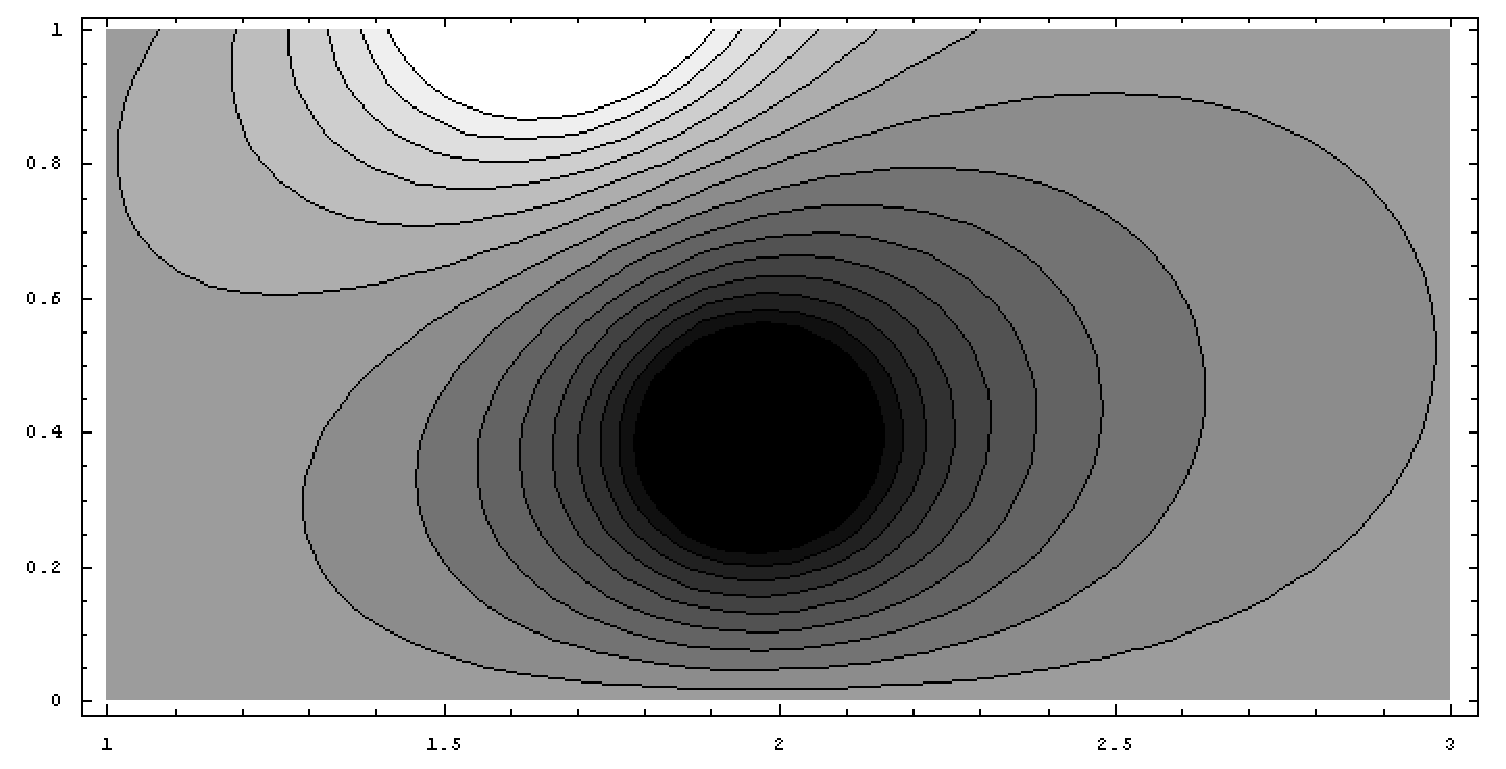
\includegraphics[width=4.9in]{img/qg_slope_n16_1src_mid.eps}
\caption{\small A solution under the QG approximation for a sloping boundary with a source in the middle.}
\label{Fig:QGSlopeFlowMid}
\end{figure}

\begin{figure}[p]
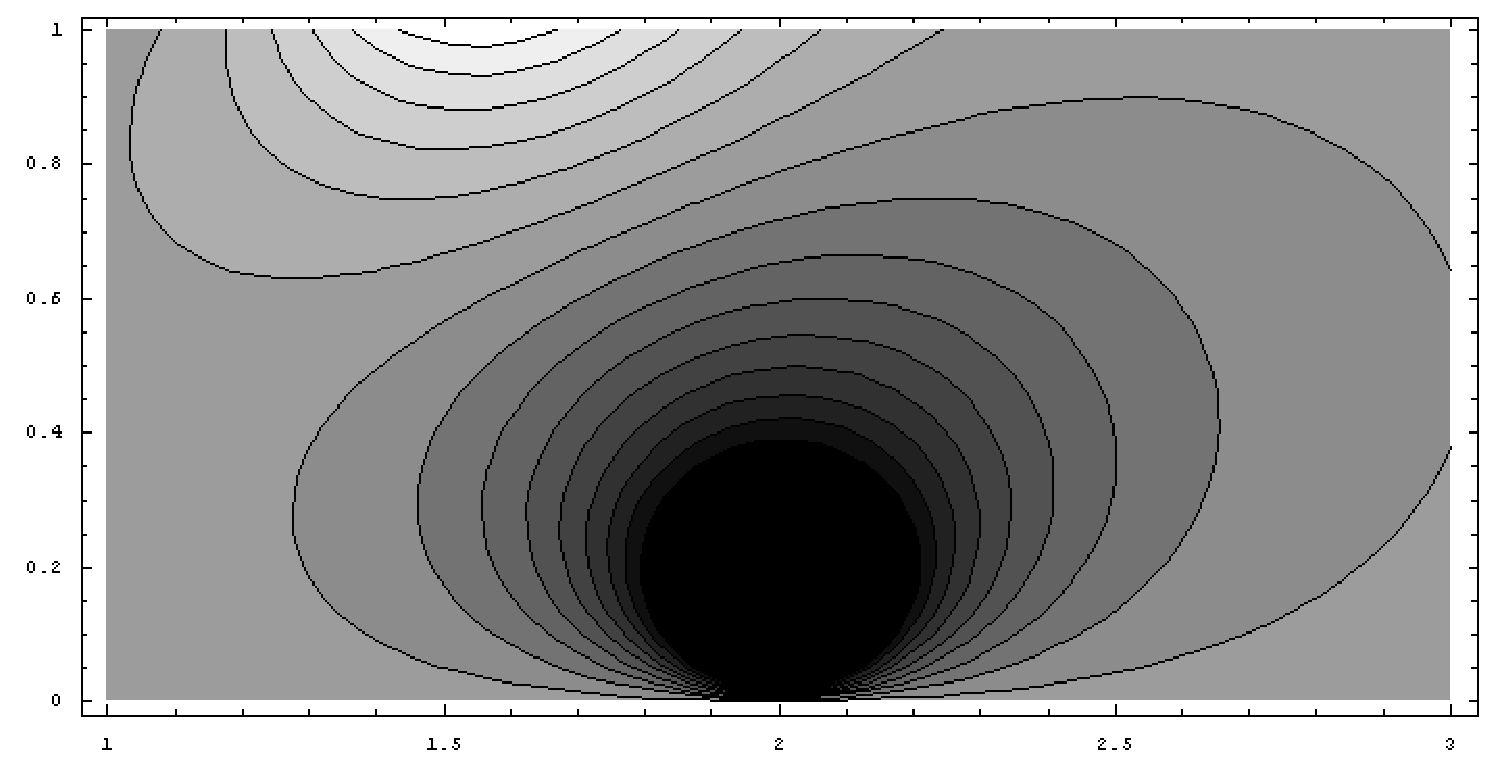
\includegraphics[width=4.9in]{img/qg_slope_n16_1src_btm.eps}
\caption{\small The same as Figure \ref{Fig:QGSlopeFlowMid}, with a source at the bottom.}
\label{Fig:QGSlopeFlowBtm}
\end{figure}

\begin{figure}[p]
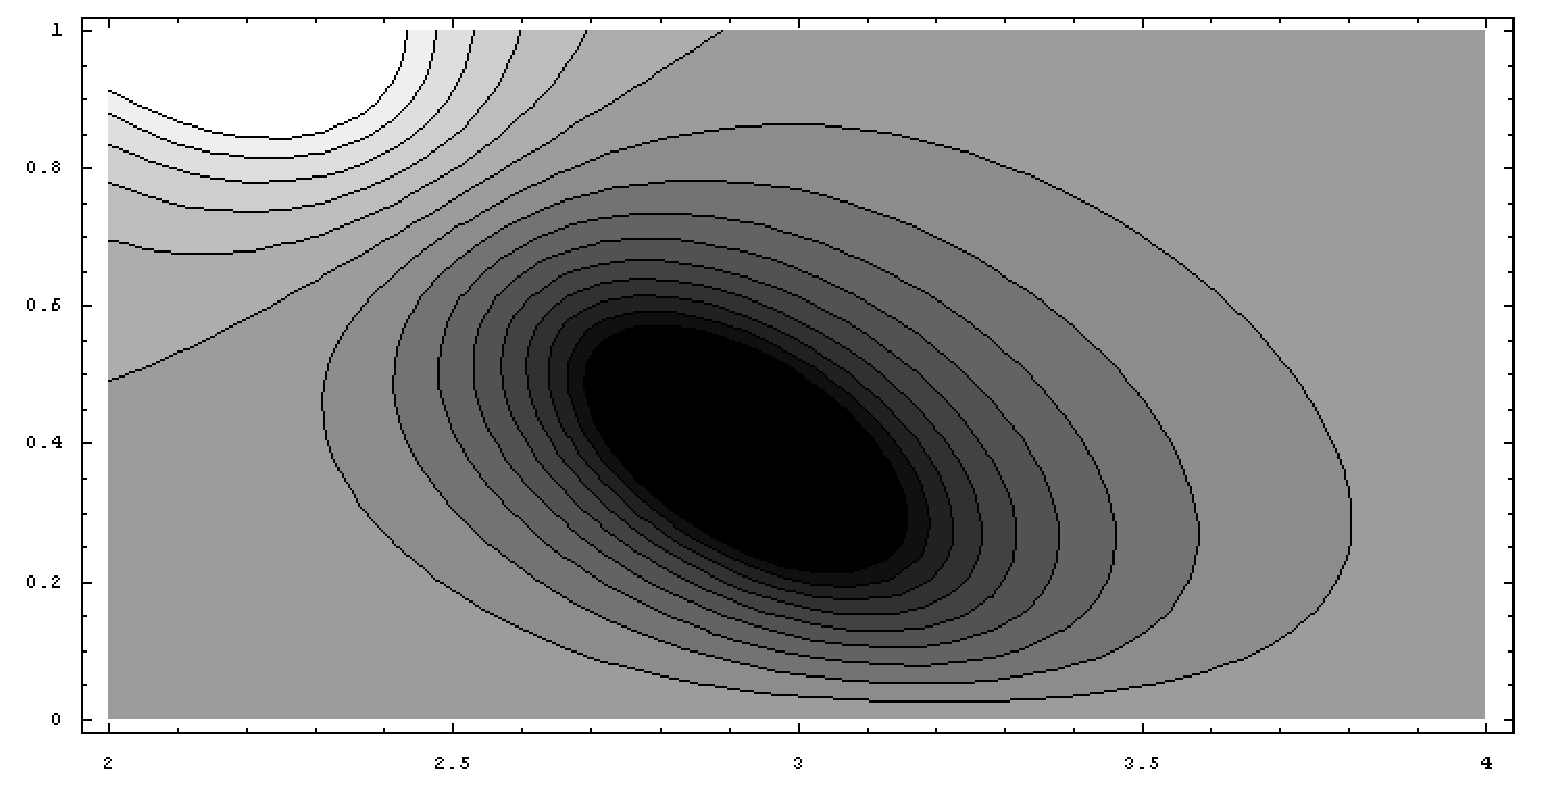
\includegraphics[width=4.9in]{img/sg_slope_n16_s075_1src_mid.eps}
\caption{\small The SG solution corresponding to Figure \ref{Fig:QGSlopeFlowMid}, with $S/F = 0.75$.}
\label{Fig:SGSlopeFlowMid}
\end{figure}

\begin{figure}[p]
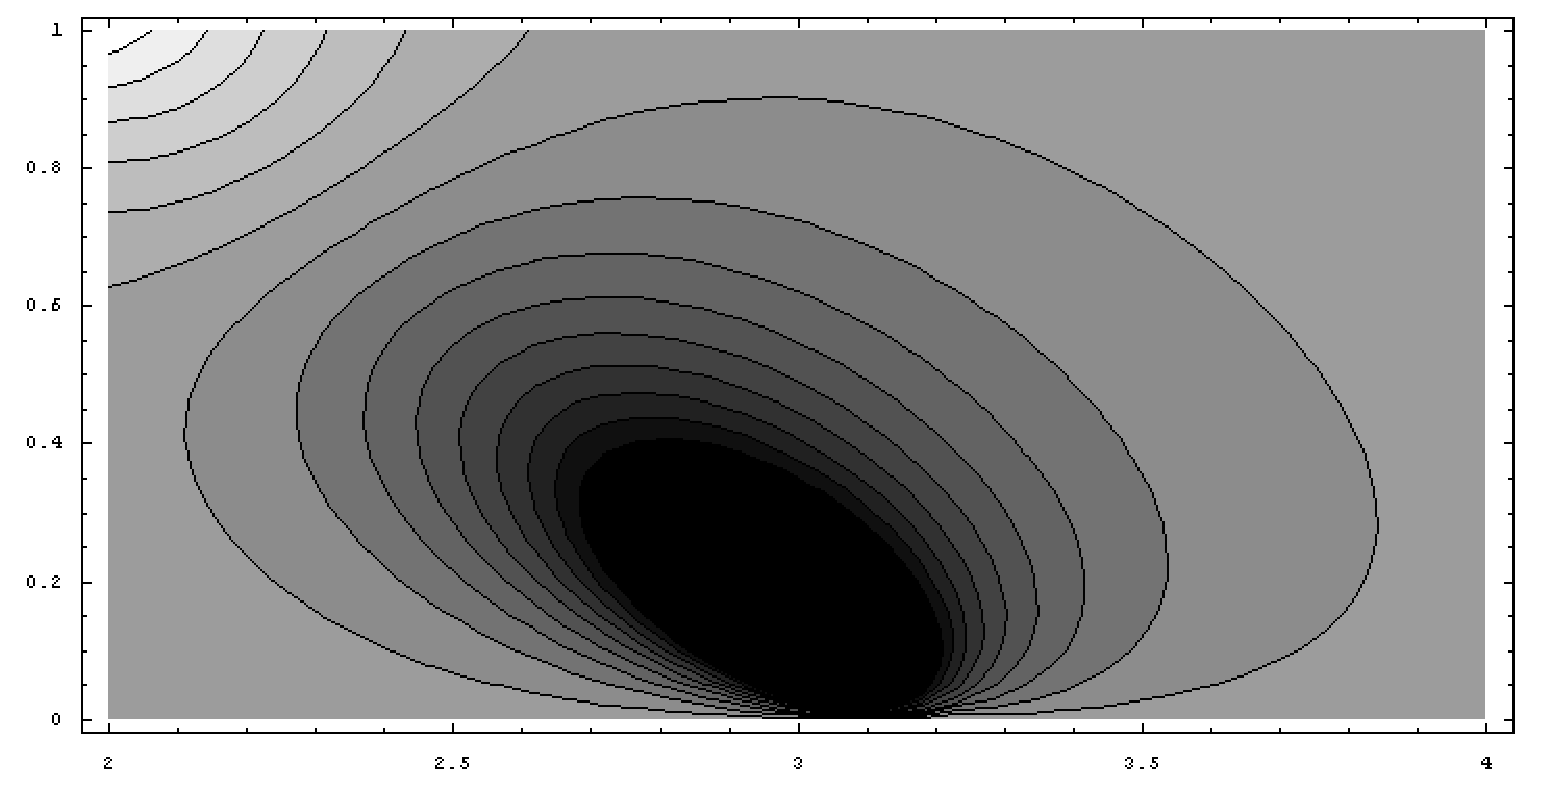
\includegraphics[width=4.9in]{img/sg_slope_n16_s075_1src_btm.eps}
\caption{\small The SG solution corresponding to Figure \ref{Fig:QGSlopeFlowMid}, with $S/F = 0.75$.}
\label{Fig:SGSlopeFlowBtm}
\end{figure}

\begin{figure}[ht]
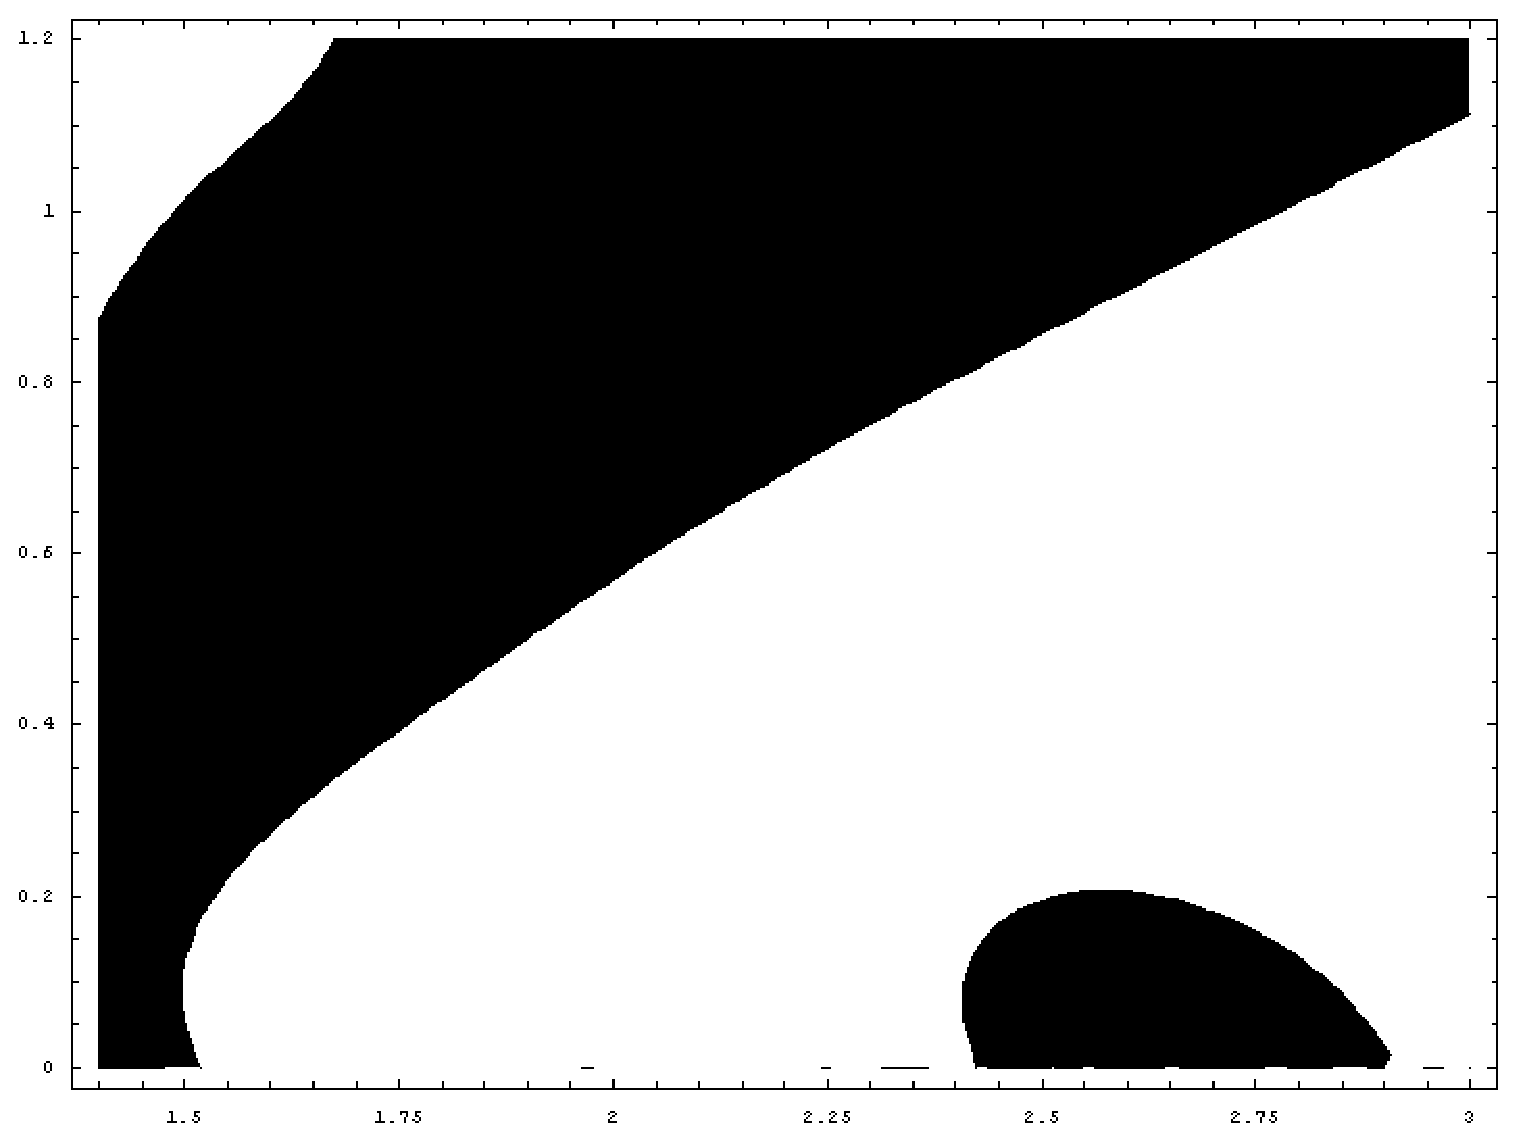
\includegraphics[width=4.9in]{img/sg_slope_2src_surface.eps}
\caption{\small The SG flow for two sources in a curved domain is solved for each source in a different wedge.}
\label{Fig:SGSlopedBoundary}
\end{figure}

The wedge problem can solved in terms of an integral. While such a solution is numerically simpler than a partial differential equation, we will focus on a restricted class of solutions where an analytic solution can be constructed in terms of elementary functions.

For cases where the wedge angle is $\theta_n = \frac{2 \pi}{n}$ for even integers $n$, the solution for $\psi$ can be constructed by the method of images. Using this method, the QG solution due to a single source such as that in Figure \ref{Fig:SlopedDomain} is found to be
\[
\psi = -\frac{Q}{\pi}\sum_{k=0}^{\frac{n}{2}-1} \log\left[\frac{\left(x-a\cos\left(\frac{4 \pi k}{n} + \gamma\right)\right)^2 + \left(z-a\sin\left(\frac{4 \pi k}{n} + \gamma\right)\right)^2}{\left(x-a\cos\left(\frac{4 \pi k}{n} - \gamma\right)\right)^2 + \left(z-a\sin\left(\frac{4 \pi k}{n} - \gamma\right)\right)^2} \right].
\]
For the SG solution, $x$ and $z$ are replaced by $X$ and $Z$, followed by the appropriate change in coordinates.

Figures \ref{Fig:QGSlopeFlowMid}--\ref{Fig:SGSlopeFlowBtm} show the streamlines for some typical sources within a sloping tropopause under both the QG and SG approximations. The image-induced flow should be neglected and replaced with a rigid upper boundary, which is a wedge in all four cases. Figure \ref{Fig:SGSlopedBoundary} demonstrates the effects of multiple sources under the SG approximation. Each source undergoes its own local transformation in order that it be a wedge in $(X,Z)$ coordinates. Since every wedge will be shifted to a different point, depending on the location of the sources, their net effect in the true coordinates will not necessarily correspond to a wedge.

%%%%%%%%%%%%%%%%%%%%%%%%%%%%%%%%%%%%%%%%%%%%%%%%%%%%%%%%%%%%%%%%%%%%%%%%%%%%%%%%
%%%%%%%%%%%%%%%%%%%%%%%%%%%%%%%%%%%%%%%%%%%%%%%%%%%%%%%%%%%%%%%%%%%%%%%%%%%%%%%%

\section{Frontal Flow for a Curved Boundary}

To model the effects of steady curvature in the tropopause, we consider the shaded domain shown in Figure \ref{Fig:CurvedDomain}.
\begin{figure}[ht]
\centering
\includegraphics{fronts_fig.4}
\caption{\small Curvature in the tropopause is modeled by the shaded region shown. The unphysical behavior on the ends will be neglected.}
\label{Fig:CurvedDomain}
\end{figure}
While such a domain is unphysical near the ends, we should be able to obtain the approximate behavior of the vertical circulation for regions close to the center. The curvature of the upper boundary is given by $a$, which sweeps an angle of $2 \theta_0$.

By means of a conformal mapping, this configuration can be converted to a domain with wedge-like boundaries, which we have already considered. We will focus on the curved upper boundary, as the transformation of the flat lower boundary is relatively straightforward.

If we project the system onto the complex plane, then the curved boundary can be parameterized as
\[ \begin{split}
w &= ae^{-i\left(\frac{\pi}{2} - \theta_0\right)} + ae^{i\left(\frac{\pi}{2} - \phi\right)} \\
  &= -ia (e^{i\theta_0} -e^{-i\phi})
\end{split} \]
for $\phi \in [-\theta_0, \theta_0]$. Now let us perform the conformal mapping $W = l^2/w$, where $l \equiv 2 a \sin \theta_0$ is the length of the bottom boundary.\footnote{Any transformation given by an analytic function is conformal, by the Cauchy-Riemann relations} This has the effect of moving points within a circle of radius $l$ to points outside the circle, followed by a reflection across the real axis. This has the additional effect of mapping a circular curve to a straight line, which we now demonstrate.

\begin{figure}[ht]
\centering
\includegraphics{fronts_fig.5}
\caption{\small Points within a circle of radius $l$ are reflected to points outside the circle by the transformation $R = l^2/r$.}
\label{Fig:CircReflection}
\end{figure}

Under this mapping, the expression for $W$ along the curve becomes
\[
W = \frac{l^2}{-ia(e^{i\theta_0} - e^{-i\phi})}.
\]

Since the endpoint $w=l$ is mapped to itself, it is helpful to remove this contribution. After some manipulation, we find that
\[
W = l - r(\phi) e^{-i\theta_0}
\]
where
\[
r(\phi) = l \left(\frac{\cos \theta_0 - \cos \phi}{1-\cos (\theta_0 + \phi)} \right).
\]
For $\phi \in [-\theta_0, \theta_0]$, this corresponds to a ray extending from $W=l$ at an angle $-\theta_0$. But for visualization purposes, we may reflect these points across the $x$-axis, as shown in Figure \ref{Fig:CircReflection}.

By solving Poisson's equation for the wedge problem in the shifted coordinates $(X',Z') = (X-l,Z)$, we obtain a solution $\widetilde{\psi}(X',Z')$ which may then be re-expressed as
\[
\psi(x,z) = \widetilde{\psi}\left(\frac{l^2 x}{x^2+z^2} - l, \frac{l^2 z}{x^2 + z^2}\right).
\]

\begin{figure}
\centering
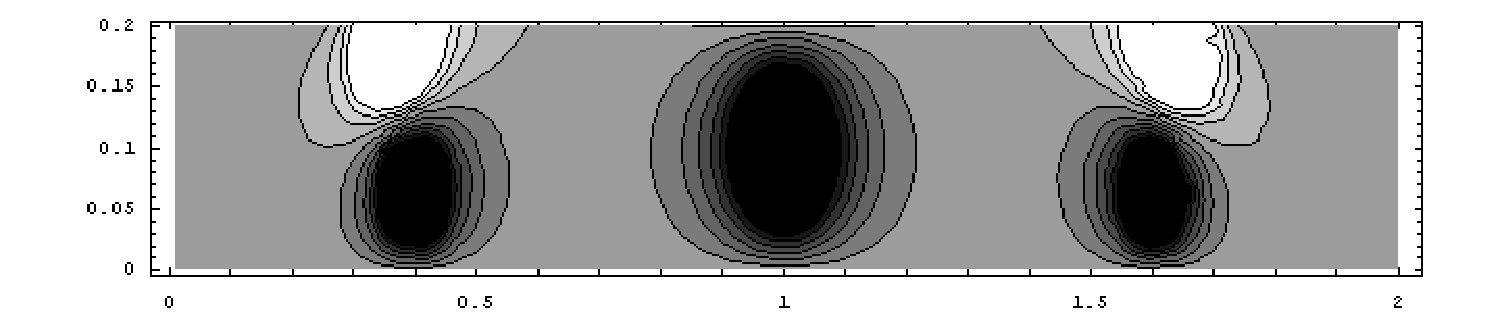
\includegraphics[width=4.9in]{img/qg_curve_n16_3src_mid.eps}
\caption{\small A solution under the QG approximation for the vertical flow for a curved upper boundary due to three sources.}
\label{Fig:QGCurvedFlow}
\end{figure}

\begin{figure}
\centering
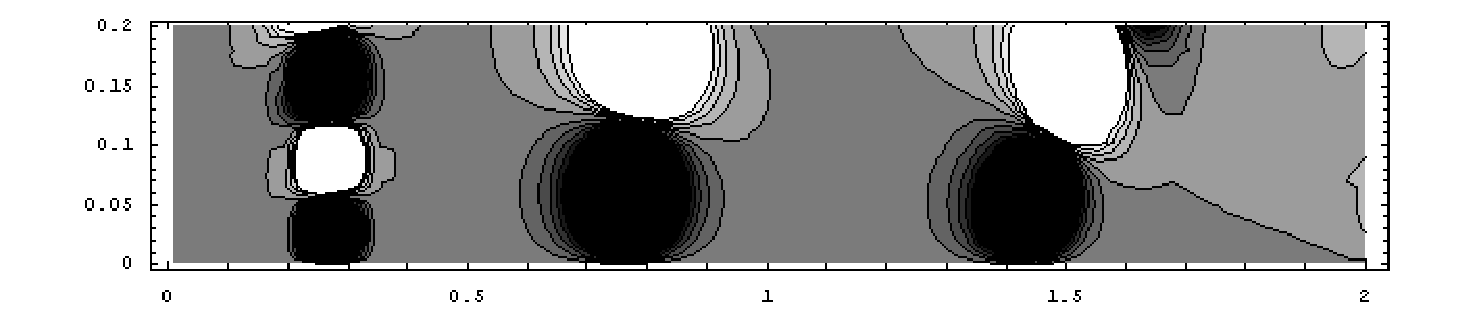
\includegraphics[width=4.9in]{img/sg_curve_n16_s075_3src_mid.eps}
\caption{\small The SG solution that transforms into the circular boundary corresponding to Figure \ref{Fig:QGCurvedFlow}, with $S/F = 0.75$.}
\label{Fig:SGCurvedFlow}
\end{figure}

\begin{figure}
\centering
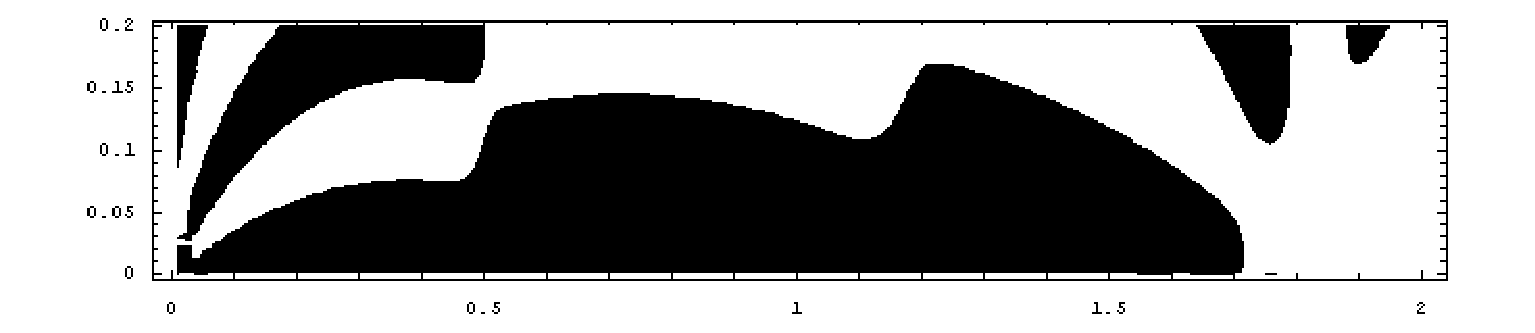
\includegraphics[width=4.9in]{img/sg_curve_3src_surface.eps}
\caption{\small The upper boundary for the SG solution in Figure \ref{Fig:SGCurvedFlow}, denoted by the largest darkened region.}
\label{Fig:SGCurvedBoundary}
\end{figure}

For the QG case, this solution corresponds to the dimensionless form of the actual streamfunction. For the SG case, a further transformation must be taken. Note however that, as with the wedge problem, circular curvature can only be solved in this way for the QG case. For the case of multiple sources, only highly irregular boundaries, as in Figure \ref{Fig:SGCurvedBoundary}, are transformed into circular upper boundaries. While analytical solutions can be obtained for the unusual domains, a circular domain under the SG approximation is presumably a much more difficult task.

%%%%%%%%%%%%%%%%%%%%%%%%%%%%%%%%%%%%%%%%%%%%%%%%%%%%%%%%%%%%%%%%%%%%%%%%%%%%%%%%
%%%%%%%%%%%%%%%%%%%%%%%%%%%%%%%%%%%%%%%%%%%%%%%%%%%%%%%%%%%%%%%%%%%%%%%%%%%%%%%%

\section{Conclusions}

We have demonstrated that it is possible to obtain analytic forms for vertical cross-front flow, as prescribed by the Sawyer-Eliassen equation, for variations from a horizontal upper boundary. Solutions for frontal flow under the QG approximation was obtained for upper boundaries that are both sloped and of constant curvature. Particular geometries of SG flow were calculated, although the surface is in general highly irregular for the case of multiple sources. The boundaries for which analytic solutions were obtained are those which are transformed into sloped and curved boundaries.

The variable upper boundary was taken to be the tropopause in a steady state, although no mention was made about the possibility of such as state occurring in nature. However, the methods described here are just as applicable for variation in topogaphy, and it may in fact be more accurate to apply them there.

It may be possible to extend these methods to higher order variations in structure. It may also be possible to approximate an arbitrary boundary through the use of splines. As a related issue, there is interest in obtaining more information behind the structure of the various SG boundaries which are transformed to wedges and circular arcs, particularly whether wedge or constant curvature boundaries can be solved in the SG case. 

Finally, in order to apply this to the true tropopause, it would be necessary to consider a model where the tropopause would react to the vertical circulation. A steady-state model may still be possible in such cases.

\bibliography{fronts}
\bibliographystyle{jas99}

\end{document}